\documentclass[11pt]{article}

\usepackage[a4paper,margin=3cm]{geometry} % For page dimensions
\usepackage{fontspec} % For font selection
\usepackage{unicode-math} % For mathematical fonts
\usepackage{polyglossia} % For language selection
\usepackage{graphicx} % For images
\usepackage[colorlinks=true, linkcolor=black, urlcolor=blue, citecolor=green]{hyperref} % For hyperlinks
\usepackage{xcolor} % Colors for code highlighting
\usepackage{fancyhdr} % For headers and footers
\usepackage{bookmark}
\usepackage{nameref}
% \usepackage{draftwatermark} % For watermarks

\usepackage{amsmath} % For mathematical equations
\usepackage{listings} % For code formattings
\usepackage{tikz} % For diagrams

\graphicspath{ {images} }

% Set fonts
% \setmainfont{Noto Serif}
\setromanfont{Noto Serif}
\setsansfont{Noto Sans}
\setmonofont{Noto Sans Mono}

% Set languages
\setmainlanguage{greek}
\setotherlanguages{english}

% Watermark
% \SetWatermarkScale{1}
% \SetWatermarkColor{gray}
% \SetWatermarkLightness{0.5}

% Header and footer settings
\pagestyle{fancy}
\setlength{\headheight}{14pt}
\fancyhf{}
\fancyhead[L]{ParkOut}
\fancyhead[R]{\leftmark} % section name
\fancyfoot[C]{\thepage}

\newcommand{\email}[1]{\href{mailto://#1}{\texttt{#1}}} % Email formatting

\begin{document}
\begin{titlepage}
    \centering
    \Huge
    ParkOut \\
    \normalsize
    \vspace{1cm}
    % TODO project logo
    % \includegraphics[width=0.5\textwidth]{upatras-logo.jpg}
    % \vspace{1cm}
    \begin{tabular}{cc}
        Γιάννης Ραβασόπουλος            & Κώστας Λουκανάρης               \\
        1100696                         & 1100610                         \\
        \email{up1100696@ac.upatras.gr} & \email{up1100610@ac.upatras.gr} \\
        \\
        Χρήστος Μάριος Νικολόπουλος     & Άγγελος Αβεντισιάν              \\
        1100644                         & 1100491                         \\
        \email{up1100644@ac.upatras.gr} & \email{up1100491@ac.upatras.gr} \\
        \\
    \end{tabular} \\
    Βασίλης Μυλωνάς \\
    1100643 \\
    \email{up1100643@ac.upatras.gr} \\
    \vspace{1.5cm}
    \Large
    \today \\
    \vspace{0.5cm}
    Τεχνολογία Λογισμικού \\
    \vspace{0.5cm}
    Τμήμα Μηχανικών Η/Υ και Πληροφορικής, \\
    Πανεπιστήμιο Πατρών \\
    \normalsize
\end{titlepage}

\newpage

\begin{abstract}
    Ανάπτυξη συστήματος και συνοδεύουσας εφαρμογής για την εύρεση/ενοικίαση
    θέσεων στάθμευσης και την διευκόλυνση συνεπιβίβασης σε κοινές διαδρομές
    (carpooling).
    Η εφαρμογή εγκαθισταται σε κινητές συσκευές και παρέχει ζωντανή πληροφόρηση
    αντλώντας πληροφορίες από τους χρήστες, στατιστικά μοντέλα και από δίκτυα
    αισθητήρων\footnote{Μελλοντική λειτουργία} όπου αυτό είναι δυνατό. Η
    εφαρμογή απευθύνεται αμφότερα σε οδηγούς αυτοκινήτων αλλά και σε πεζούς.
    Στόχος είναι η καλύτερη αξιοποίηση του οδικού δικτύου και η μείωση της
    κυκλοφοριακής συμφόρησης σε αστικές περιοχές.
\end{abstract}

\newpage

\tableofcontents

\newpage

\section{Σύσταση Ομάδας}

Η ομάδα αποτελείται από 5 μέλη:

\begin{itemize}
    \item Βασίλης Μυλωνάς (Επικεφαλής Έργου/Project Manager)
    \item Άγγελος Αβεντισιάν (Υπεύθυνος Ποιότητας/QA Manager)
    \item Γιάννης Ραβασόπουλος
    \item Κώστας Λουκανάρης
    \item Χρήστος Μάριος Νικολόπουλος
\end{itemize}

Η επιλογή των ρόλων έγινε με βάση την εμπειρία και τα ενδιαφέροντα του κάθε
μέλους έπειτα από ψηφοφορία.

\newpage

\section{Περιγραφή}

\subsection{Το Πρόβλημα της Κυκλοφοριακής Συμφόρησης}

\subsubsection{Η Επιλογή του Αυτοκινήτου έναντι των ΜΜΜ}

Είναι γνωστό ότι το μεγαλύτερο μέρος του αστικού πληθυσμού είναι άτομα τα
οποία έχουν καθημερινές υποχρεώσεις και πρέπει να βρίσκονται
σε συγκεκριμένα μέρη σε συγκεκριμένες ώρες όπως φοιτητές και εργαζόμενοι.
Είναι εύκολο να δει κανείς πως τα περισσότερα από αυτά τα άτομα
έχουν κοινό προορισμό και μάλιστα μετακινούνται και σε κοινές ώρες της
ημέρας.

Ανάμεσα στον μεγάλο αριθμό ατόμων με κοινό προορισμό πολλοί επιλέγουν
την αυτοκίνηση λόγω της κακής κατάστασης των μέσων μαζικής μεταφοράς.
Χαρακτηριστικό παράδειγμα είναι τα λεωφορεία με δρομολόγια προς το
πανεπιστήμιο τα οποία είναι γεμάτα τις πρωινές ώρες.
Η αύξηση της χρήσης των αυτοκινήτων οδηγεί σε αύξηση της
κυκλοφοριακής συμφόρησης και της ρύπανσης.

\subsubsection{Η Έλλειψη Χώρου Στάθμευση στα Κέντρα των Πόλεων}

Ένα παράλληλο πρόβλημα είναι η έλλειψη θέσεων στάθμευσης στο κέντρο
των πόλεων όπου ο χώρος είναι περιορισμένος και οι οδηγοί καταφεύγουν
σε παράνομες πρακτικές όπως η διπλοπαρκάρισμα ή η στάθμευση σε
πεζοδρόμια. Αυτό επιβαρύνει την κυκλοφοριακή ροή καθώς μειώνεται
το αποτελεσματικό πλάτος των δρόμων και δημιουργούνται καθυστερήσεις
κατά τη διέλευση μεγάλων οχημάτων όπως λεωφορεία και τα φορτηγά.

Είναι εμφανές ότι αυτά τα δύο φαινόμενα είναι αλληλένδετα και
τροφοδοτούν το ένα το άλλο. Η βελτίωση της κατάστασης απαιτεί
συνδυαστική προσέγγιση και των δύο προβλημάτων και δυστυχώς δεν
υπάρχει κατάλληλος ρυθμός ανάπτυξης των υποδομών για να
αντιμετωπιστούν αυτά τα προβλήματα.

\subsection{Λειτουργίες της Εφαρμογής}

Η εφαρμογή ParkOut στοχεύει στην επίλυση
και των δύο αυτών προβλημάτων συνδυάζοντας την λειτουργία του carpooling
με την εύρεση καλύτερων θέσεων στάθμευσης.

\subsubsection{Carpooling και Συνδυασμός Διαδρομών}

Η εφαρμογή θα επιτρέπει στους χρήστες να δηλώνουν τις δραστηριότητες τους
και να αναζητήσουν άλλους χρήστες που πηγαίνουν στον ίδιο προορισμό.
Μέσου αυτού του μηχανισμού οι χρήστες θα μπορούν να μοιράζονται το
ίδιο όχημα και να μειώνουν το κόστος της μεταφοράς τους καθώς και το
περιβαλλοντικό τους αποτύπωμα ενώ ταυτόχρονα θα μειώνεται η κυκλοφοριακή
φόρτιση στους δρόμους.

\subsubsection{Εύρεση Θέσεων Στάθμευσης}

Η εφαρμογή θα παρέχει επίσης πληροφορίες για διαθέσιμες θέσεις
στάθμευσης σε δημόσιους και ιδιωτικούς χώρους. Οι χρήστες θα
μπορούν να δηλώνουν ελεύθερες θέσεις στάθμευσης και να τις μοιράζονται με
άλλους χρήστες της εφαρμογής. Επιπλέον αυτού θα δίνεται η δυνατότητα να
ενοικιάζουν θέσεις στάθμευσης σε ιδιωτικούς χώρους στάθμευσης ή σε θέσεις
με παρκόμετρα και να πληρώνουν για την στάθμευση τους μέσω της εφαρμογής.
Στόχος είναι η καλύτερη αξιοποίηση του οδικού δικτύου για τη στάθμευση
των αυτοκινήτων και η μείωση της συγκέντρωσης σταθμευμένων οχημάτων σε
πολυσύχναστους δρόμους.

\subsection{Σενάρια}

Ο χρήστης κατεβάζει την εφαρμογή από το Play Store ή το App Store.
Έπειτα δημιουργεί έναν λογαριασμό μέσω email, Google ή Facebook.
Αφού συνδεθεί στην εφαρμογή μπορεί να δηλώσει τις δραστηριότητες του.

Η έννοια της δραστηριότητας είναι γενική και μπορεί να αφορά οτιδήποτε
από την εργασία του χρήστη, την σχολή του ή κάποια άλλη υποχρέωση.
Συγκεκριμένα δηλώνει μια τοποθεσία και τις ώρες άνα μέρα της εβδομάδας
για κάθε δραστηριότητα. Επιπλέον δηλώνει εάν διαθέτει όχημα ή όχι.

Έχοντας δηλώσει την δραστηριότητα του μπορεί να αναζητήσει άλλους χρήστες
οι οποίοι έχουν δηλώσει όμοιες
\footnote{
    Η έννοια της ομοιότητας αποτελεί σχεδιαστική λεπτομέρεια αλλά
    αναμένεται να βασίζεται σε γεωγραφικές αποστάσεις και χρονικές διαφορές.
}
δραστηριότητες και να κανονίσει να μοιραστεί ένα όχημα μαζί τους για
την κοινή τους διαδρομή.

Ένας εκ των χρηστών που διαθέτουν όχημα επιλέγεται
ως ο οδηγός της διαδρομής και οι υπόλοιποι ως επιβάτες. Ο οδηγός μπορεί να
επιλέξει να μοιραστεί το κόστος της διαδρομής με τους επιβάτες. Οι
επιβάτες μπορούν να αποδεχτούν ή να απορρίψουν την προσφορά του οδηγού.
Στην οποία περίπτωση η διαδικασία επαναλαμβάνεται.
Αφού συμφωνηθεί η συνεπιβίβαση επιλέγονται η ώρα και το σημείο συνάντησης
για την παραλαβή των επιβατών μέσω της εφαρμογής.

Σε κάθε παράληψη επιβάτη υπάρχει επιβεβαίωση μέσω της εφαρμογής και ο
οδηγός λαμβάνει προσωρινά πόντους για την επιβράβευση του οι οποίοι
μονιμοποιούνται όταν ολοκληρωθεί η διαδρομή.

Αφού ολοκληρωθεί η διαδρομή οι επιβάτες μπορούν να βαθμολογήσουν τον
οδηγό και να αφήσουν σχόλια για την κατάσταση του οχήματος και την
συμπεριφορά του οδηγού. Ομοίως ο οδηγός μπορεί να βαθμολογήσει τους
επιβάτες.

\newpage

\section{Domain Model}

\begin{description}
    \item[User]
        Οποιοσδήποτε χρήστης της εφαρμογής. Με αυτόν τον όρο περιγράφουμε
        οποιοδήποτε άτομο, επιχείρηση ή άλλη οντότητα που αξιοποιεί τις
        υπηρεσίες της εφαρμογής.
    \item[Driver]
        Ένας χρήστης της εφαρμογής ο οποίος οδηγεί κάποιο όχημα.
    \item[Vehicle]
        Ένα όχημα που χρησιμοποιείται για μετακίνηση από κάποιον οδηγό της
        εφαρμογής.
    \item[ParkingSpace]
        Ένας γενικευμένος χώρος στάθμευσης. Μπορεί να είναι δημόσιος ή ιδιωτικός
        π.χ. ένα τμήμα δρόμου, ένα γκαράζ που νοικιάζει κάποιος ή ένας υπόγειος
        χώρος.
    \item[ParkingSpot]
        Μια συγκεκριμένη θέση στάθμευσης. Μπορεί να είναι διαθέσιμη,
        κατειλημμένη ή σε άγνωστη κατάσταση. Μια θέση στάθμευσης είναι πάντα
        μέρος ενός χώρου στάθμευσης.
    \item[ParkingReservation]
        Μια κράτηση μιας θέσης στάθμευσης. Αφορά κυρίως ιδιωτικούς χώρους
        στάθμευσης. Eίναι έναντι πληρωμής και μπορεί να είναι
        προγραμματισμένη ή άμεση.
    \item[ParkingSpaceOwner]
        Ένας χρήστης της εφαρμογής ο οποίος είναι ιδιοκτήτης ενός χώρου
        στάθμευσης και το έχει δηλώσει μέσω της εφαρμογής. Μπορεί να
        είναι ιδιώτης ή κάποια επιχείρηση π.χ. ένας
        ιδιοκτήτης πολυκατοικίας ο οποίος ενοικιάζει τον υπόγειο χώρο στάθμευσης
        σε τρίτους μέσω της εφαρμογής ή μια εταιρεία που διαχειρίζεται ένα
        πολυόροφο χώρο στάθμευσης.
    \item[Payment]
        Μια πληρωμή που πραγματοποιείται μέσω της εφαρμογής. Ενδεικτικά μπορεί
        να αφορά την ενοικίαση μιας θέσης στάθμευσης ή την αγορά ενός
        εισιτηρίου για παρκόμετρο.
    \item[Rating]
        Η βαθμολογία που δίνει ένας χρήστης σε έναν άλλο χρήστη. Μπορεί να
        αφορά την συμπεριφορά του χρήστη ή την κατάσταση ενός χώρου
        στάθμευσης. Μπορεί να περιλαμβάνει σχόλια και εικόνες.
    \item[Report]
        Μια αναφορά που κάνει ένας χρήστης σε έναν άλλο χρήστη για να
        καταγγείλει παράνομη η ανεπιθύμητη δραστηριότητα. Περιλαμβάνει
        κείμενο και έναν λόγο αναφοράς.
    \item[Location]
        Μια γεωγραφική τοποθεσία, περιλαμβάνει διεύθυνση ή συντεταγμένες.
    \item[Route]
        Μια διαδρομή από ένα σημείο Α σε ένα σημείο Β. Μπορεί να περιλαμβάνει
        σημεία στάσης.
    \item[Ride]
        Αντιπροσωπεύει μια συνεπιβίβαση. Ένας οδηγός εκτελώντας μια διαδρομή
        μπορεί να μεταφέρει περισσότερους από έναν επιβάτες οι οποίοι έχουν
        κοινό προορισμό.
    \item[Pickup]
        Αντιπροσωπεύει την παραλαβή ενός επιβάτη από τον οδηγό. Περιλαμβάνει
        σημείο συνάντησης και ώρα.
    \item[Carpooler]
        Ένας χρήστης της εφαρμογής ο οποίος δεν οδηγεί κάποιο όχημα αλλά
        χρησιμοποιεί τις υπηρεσίες της εφαρμογής για να βρει οδηγούς που πάνε
        στο ίδιο μέρος με αυτόν.
    \item[Area]
        Μια περιοχή (πχ ένας δήμος).
    \item[Reward]
        Μια επιβράβευση η οποία δίνεται σε έναν χρήστη με βάση την χρήση της
        εφαρμογής. Για παράδειγμα ένας οδηγός που μεταφέρει πολλούς επιβάτες
        μπορεί να λάβει ένα κουπόνι έκπτωσης 15\% σε κάποιον φούρνο.
    \item[Activity]
        Μια δραστηριότητα είναι κάτι το οποίο θέλει να κάνει ο χρήστης σε
        συγκεκριμένο μέρος και ώρα και για το οποίο χρειάζεται μεταφορικό μέσο.
\end{description}

\begin{figure}
    \centering
    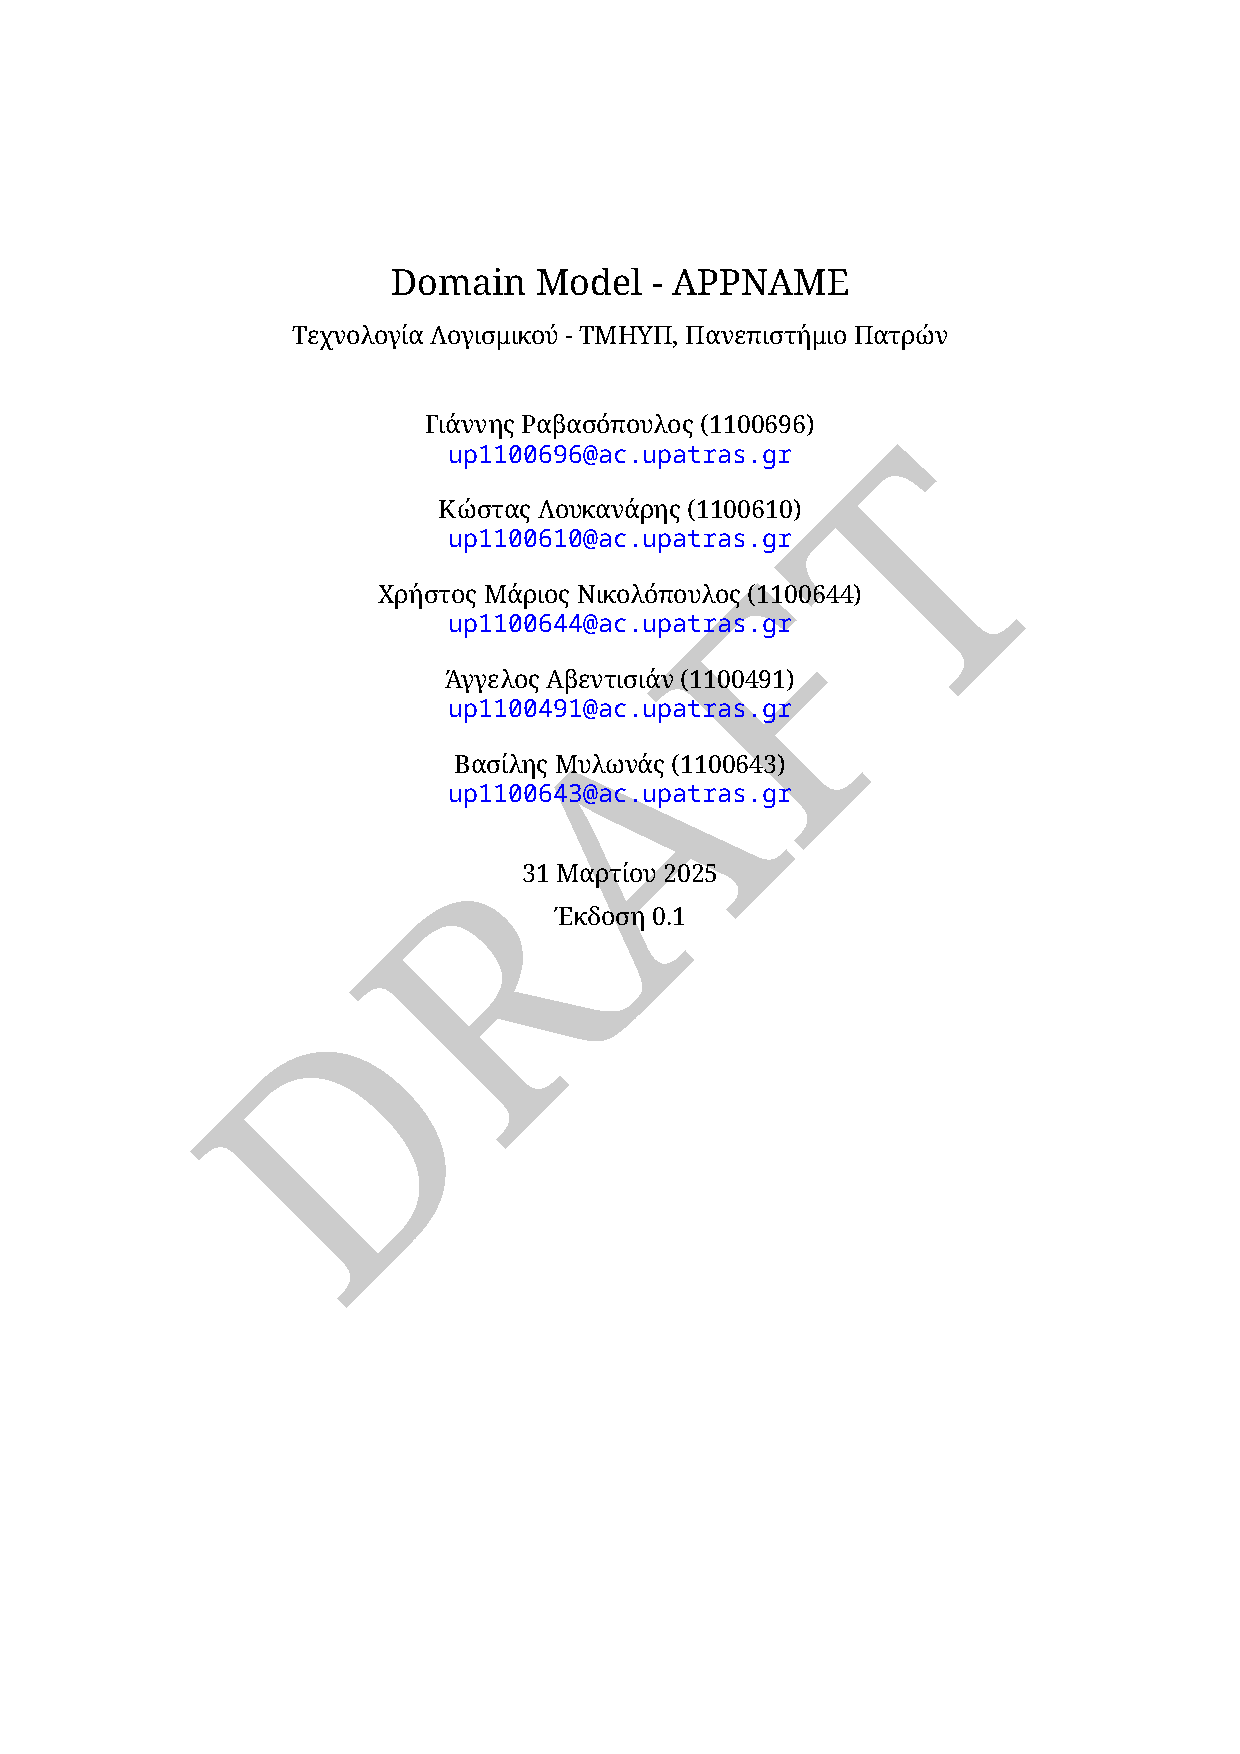
\includegraphics[width=\textwidth]{domain-model}
    \caption{Domain Model}
\end{figure}

\newpage

\section{Use Cases}

% Carpooling (Aggelos-Yannis)
\subsection{Find Ride}

Ο χρήστης επιθυμεί να βρεί οδηγό με κοινή διαδρομή με αυτόν για να συμμετέχει σε
κάποια δραστηριότητα (εργασία, μάθημα κλπ).

\subsubsection{Βασική Ροή}
\begin{enumerate}
    \item Ο χρήστης επιλέγει "Find Ride"
    \item Η εφαρμογή εμφανίζει τις δραστηριότητες του χρήστη.
    \item Ο χρήστης επιλέγει μια δραστηριότητα.
    \item To σύστημα εκτελεί αναζήτηση με βάση τα κριτήρια του χρήστη για δραστηριότητες
          άλλων χρηστών που εμφανίζουν τοπική και χρονική ομοιότητα.
    \item Το σύστημα κατατάσει τις δραστηριότητες με βάση την ομοιότητα.
    \item Το σύστημα εμφανίζει τις δραστηριότητες που βρέθηκαν.
    \item Ο χρήστης επιλέγει μια δραστηριότητα.
    \item Το σύστημα εμφανίζει τα στοιχεία του χρήστη που έχει δηλώσει την δραστηριότητα.
    \item Ο χρήστης επιλέγει "Pool".
    \item Το σύστημα ειδοποιεί τον δέκτη και ο χρήστης περιμένει την επιβεβαίωση του.
    \item O δέκτης αποδέχεται την πρόταση του χρήστη.
    \item Το σύστημα ενημερώνει τον χρήστη για τον επιτυχή προγραμματισμό.
\end{enumerate}

\subsubsection{Εναλλακτική Ροή: Ακύρωση 1}

\begin{enumerate}
    \item[3] Ο χρήστης ακυρώνει την αναζήτηση και επιστρέφει στην αρχική οθόνη.
\end{enumerate}

\subsubsection{Εναλλακτική Ροή: Ακύρωση 2}

\begin{enumerate}
    \item[7] Ο χρήστης ακυρώνει την αναζήτηση και επιστρέφει στην αρχική οθόνη.
\end{enumerate}

\subsubsection{Εναλλακτική Ροή: Ακύρωση 3}

\begin{enumerate}
    \item[9] Ο χρήστης αλλάζει γνώμη και πατάει "επιστροφή".
    \item[10] Συνέχεια από το βήμα 6 της βασικής ροής.
\end{enumerate}

\subsubsection{Εναλλακτική Ροή: Απόρριψη Πρότασης}

\begin{enumerate}
    \item[11] Ο δέκτης απορρίπτει την πρόταση του χρήστη.
    \item[12] Συνέχεια από το βήμα 6 της βασικής ροής.
\end{enumerate}

\subsubsection{Εναλλακτική Ροή: Εσωτερικό Σφάλμα}

\begin{enumerate}
    \item[5] Προκύπτει εσωτερικό σφάλμα κατά την αναζήτηση.
    \item[6] Το σύστημα ενημερώνει τον χρήστη για το σφάλμα και προτρέπει τον
        χρήστη σε αναφορά σφάλματος.
\end{enumerate}

\subsubsection{Εναλλακτική Ροή: Ο χρήστης δεν έχει δραστηριότητες}

\begin{enumerate}
    \item[2] Η εφαρμογή προτείνει την δημιουργία μιας δραστηριότητας.
    \item[3] Συνέχεια από το βήμα 1 της βασικής ροής του "Create Activity".
\end{enumerate}

\subsubsection{Εναλλακτική Ροή: Δεν βρέθηκαν όμοιες δραστηριότητες}

\begin{enumerate}
    \item[5] Το σύστημα δεν βρίσκει καμία δραστηριότητα που να ταιριάζει με τα
        κριτήρια του χρήστη.
    \item[6] Το σύστημα ενημερώνει τον χρήστη για την αποτυχία και προτείνει
        τροποποίηση της δραστηριότητας ή τη χρήση δημόσιας συγκοινωνίας.
    \item[7] Ο χρήστης επιλέγει "ΟΚ" και επιστρέφει στην αρχική οθόνη.
\end{enumerate}


\subsection{Create Activity}

Ο χρήστης επιθυμεί να δημιουργήσει μια δραστηριότητα στην εφαρμογή.

\subsubsection{Βασική Ροή}

\begin{enumerate}
    \item Ο χρήστης επιλέγει "Create Activity"
    \item Η εφαρμογή δημιουργεί μια κενή δραστηριότητα και την αποθηκεύει
          προσωρινά.
    \item Συνέχεια από το βήμα 2 της βασικής ροής του use case "Edit Activity".
\end{enumerate}


\subsubsection{Edit Activity}

\begin{enumerate}
    \item Ο χρήστης επιλέγει "Edit Activity".
    \item Η εφαρμογή εμφανίζει μενού με επιλογές για την ιδιότητα του χρήστη (πχ φοιτητής).
    \item Ο χρήστης επιλέγει την ιδιότητα του.
    \item Η εφαρμογή εμφανίζει την φόρμα αναζήτησης και έναν χάρτη της περιοχής του χρήστη.
    \item Ο χρήστης δηλώνει την περιοχή στην οποία επιθυμεί να μετακινηθεί.
    \item Η εφαρμογή εμφανίζει μενού με επιλογές για τις μέρες και τις ώρες έναρξης και λήξης
          της δραστηριότητας.
    \item Ο χρήστης εισάγει τα κατάλληλα στοιχεία.
    \item H εφαρμογή εμφανίζει μενού με επιλόγες για το μέσο μεταφοράς του χρήστη
    \item Ο χρήστης επιλέγει το μέσο μεταφοράς του.
    \item Το σύστημα εκτελεί προεπεξεργασία στα δεδομένα.
    \item Το σύστημα εισάγει την δραστηριότητα στο κατάλογο δραστηριοτήτων του χρήστη.
    \item Η εφαρμογή εμφανίζει μήνυμα επιτυχίας.
\end{enumerate}

\subsubsection{Εναλλακτική Ροή: Ακύρωση 1}

\begin{enumerate}
    \item[3] Ο χρήστης ακυρώνει την διαδικασία και επιστρέφει στην αρχική οθόνη.
\end{enumerate}

\subsubsection{Εναλλακτική Ροή: Ακύρωση 2}

\begin{enumerate}
    \item[5] Ο χρήστης ακυρώνει την διαδικασία και επιστρέφει στην αρχική οθόνη.
\end{enumerate}

\subsubsection{Εναλλακτική Ροή: Ακύρωση 3}

\begin{enumerate}
    \item[7] Ο χρήστης ακυρώνει την διαδικασία και επιστρέφει στην αρχική οθόνη.
\end{enumerate}

\subsubsection{Εναλλακτική Ροή: Ακύρωση 4}

\begin{enumerate}
    \item[9] Ο χρήστης ακυρώνει την διαδικασία και επιστρέφει στην αρχική οθόνη.
\end{enumerate}

\subsubsection{Εναλλακτική Ροή: Μη έγκυρα στοιχεία}

\begin{enumerate}
    \item[7] Ο χρήστης εισάγει μη έγκυρα στοιχεία.
    \item[8] Το σύστημα εμφανίζει μήνυμα σφάλματος και ζητά διόρθωση.
    \item[9] Συνέχεια από το βήμα 6 της βασικής ροής.
\end{enumerate}


% Carpooling (Kwstas-Creezy)
\include{tex/use-cases/find-parking}

% Billy Mylo
\subsection{Manage Parking Spaces}
\label{uc:manage-parking-spaces}

Ο χρήστης επιθυμεί να διαχειριστεί τα \textit{ParkingSpaces} που έχει δηλώσει
ή να δηλώσει καινούρια.

\subsubsection{Βασική Ροή: Αλλαγή στοιχείων κάποιου \textit{ParkingSpace}}

\begin{enumerate}
    \item[1] Ο χρήστης επιλέγει "Manage Parking Spaces".
    \item[2] Η εφαρμογή εμφανίζει μια λίστα με τα \textit{ParkingSpaces} που έχει
        δηλώσει ο χρήστης.
    \item[3] Ο χρήστης επιλέγει το \textit{ParkingSpace} που θέλει να διαχειριστεί.
    \item[4] Η εφαρμογή εμφανίζει τα στοιχεία του \textit{ParkingSpace} καθώς και
        στατιστικά σχετικά με τις ενοικιάσεις.
    \item[5] Ο χρήστης επιλέγει "Edit" για να τροποποιήσει τα στοιχεία του
        \textit{ParkingSpace}.
    \item[6] Καλείται η περίπτωση χρήσης \nameref{uc:edit-parking-space}
\end{enumerate}

\subsubsection{Εναλλακτική Ροή: Έξοδος}

\begin{enumerate}
    \item[3] Ο χρήστης επιλέγει το πλήκτρο επιστροφής.
    \item[4] Η εφαρμογή επιστρέφει στην κεντρική οθόνη.
\end{enumerate}

\subsubsection{Εναλλακτική Ροή: Δεν υπάρχουν δηλωμένα \textit{ParkingSpaces}}

\begin{enumerate}
    \item[2] Η εφαρμογή εμφανίζει μήνυμα ότι δεν υπάρχουν δηλωμένα
        \textit{ParkingSpaces}.
    \item[3] Ο χρήστης επιλέγει "+".
    \item[4] Καλείται η περίπτωση χρήσης \nameref{uc:register-parking-space}
\end{enumerate}

\subsubsection{Εναλλακτική Ροή: Δήλωση \textit{ParkingSpace}}

\begin{enumerate}
    \item[3] Ο χρήστης επιλέγει "+".
    \item[4] Καλείται η περίπτωση χρήσης \nameref{uc:register-parking-space}.
\end{enumerate}

\newpage

\subsection{Register Parking Space}
\label{uc:register-parking-space}

Ο χρήστης επιθυμεί να δηλώσει ένα \textit{ParkingSpace} προς ενοικίαση.

\subsubsection{Βασική Ροή: Δήλωση \textit{ParkingSpace}}

\begin{enumerate}
    \item[1] Η εφαρμογή εμφανίζει την φόρμα δήλωσης.
    \item[2] Ο χρήστης συμπληρώνει τα στοιχεία του \textit{ParkingSpace},
        ενδεικτικά ώρες λειτουργίας, τιμή ενοικίασης και διεύθυνση.
    \item[3] Ο χρήστης επισυνάπτει φωτογραφίες του \textit{ParkingSpace} και έγγραφα
        για να πιστοποιήσει την ιδιοκτησία του.
    \item[4] Ο χρήστης επιλέγει "Submit".
    \item[5] Η εφαρμογή ελέγχει την εγκυρότητα των στοιχείων.
    \item[6] Η εφαρμογή αποθηκεύει τα στοιχεία του \textit{ParkingSpace}.
    \item[7] Η εφαρμογή εμφανίζει μήνυμα σχετικά με την επιτυχία της διαδικασίας.
    \item[8] Η εφαρμογή επιστρέφει στην οθόνη \nameref{uc:manage-parking-spaces}.
\end{enumerate}

\subsubsection{Εναλλακτική Ροή: Ακύρωση}

\begin{enumerate}
    \item[4] Ο χρήστης επιλέγει "Cancel".
    \item[5] Η εφαρμογή επιστρέφει στην οθόνη \nameref{uc:manage-parking-spaces}.
\end{enumerate}

\subsubsection{Εναλλακτική Ροή: Απόρριψη Δήλωσης 1}

\begin{enumerate}
    \item[6] Το σύστημα απορρίπτει την δήλωση \textit{ParkingSpace}.
    \item[7] Η εφαρμογή εμφανίζει μήνυμα απόρριψης και ζητάει από τον χρήστη να
        διορθώσει τα στοιχεία.
    \item[8] Ο χρήστης διορθώνει τα στοιχεία και επιλέγει "Submit".
    \item[9] Συνέχεια από το βήμα 7 της βασικής ροής.
\end{enumerate}

\subsubsection{Εναλλακτική Ροή: Απόρριψη Δήλωσης 2}

\begin{enumerate}
    \item[6] Το σύστημα απορρίπτει την δήλωση \textit{ParkingSpace}.
    \item[7] Η εφαρμογή εμφανίζει μήνυμα απόρριψης και ζητάει από τον χρήστη να
        διορθώσει τα στοιχεία.
    \item[8] Ο χρήστης επιλέγει "Cancel".
    \item[9] Η εφαρμογή επιστρέφει στην οθόνη \nameref{uc:manage-parking-spaces}.
\end{enumerate}

\newpage

\subsection{Edit Parking Space}
\label{uc:edit-parking-space}

Ο χρήστης επιθυμεί να αλλάξει τα στοιχεία του \textit{ParkingSpace} που έχει
δηλώσει.

\subsubsection{Βασική Ροή}

\begin{enumerate}
    \item[1] Η εφαρμογή εμφανίζει μια φόρμα με τα επεξεργάσιμα στοιχεία του
        \textit{ParkingSpace}.
    \item[2] Ο χρήστης αλλάζει τα στοιχεία του \textit{ParkingSpace} και
        επιλέγει "Confirm".
    \item[3] Το σύστημα αποθηκεύει τις αλλαγές.
    \item[4] Η εφαρμογή επιστρέφει στην οθόνη \nameref{uc:manage-parking-spaces}.
\end{enumerate}

\subsubsection{Εναλλακτική Ροή: Διαγραφή \textit{ParkingSpace} 1}

\begin{enumerate}
    \item[2] Ο χρήστης επιλέγει "Delete".
    \item[3] Η εφαρμογή ζητάει επιβεβαίωση διαγραφής.
    \item[4] Ο χρήστης επιλέγει "Confirm".
    \item[5] Το σύστημα αφαιρεί το \textit{ParkingSpace} από την λίστα των
        διαθέσιμων \textit{ParkingSpaces} και το διαγράφει.
    \item[6] Η εφαρμογή επιστρέφει στην οθόνη \nameref{uc:manage-parking-spaces}.
\end{enumerate}

\subsubsection{Εναλλακτική Ροή: Διαγραφή \textit{ParkingSpace} 2}

\begin{enumerate}
    \item[2] Ο χρήστης επιλέγει "Delete".
    \item[3] Η εφαρμογή ζητάει επιβεβαίωση διαγραφής.
    \item[4] Ο χρήστης επιλέγει "Cancel".
    \item[5] Η εφαρμογή επιστρέφει στην οθόνη \nameref{uc:edit-parking-space}.
\end{enumerate}

\subsubsection{Εναλλακτική Ροή: Απενεργοποίηση \textit{ParkingSpace}}

\begin{enumerate}
    \item[2] Ο χρήστης επιλέγει "απενεργοποίηση".
    \item[3] Το σύστημα αφαιρεί το \textit{ParkingSpace} από την λίστα των
        διαθέσιμων \textit{ParkingSpaces}.
    \item[4] Η εφαρμογή επιστρέφει στην οθόνη \nameref{uc:edit-parking-space}.
\end{enumerate}

\subsubsection{Εναλλακτική Ροή: Ενεργοποίηση \textit{ParkingSpace}}

\begin{enumerate}
    \item[2] Ο χρήστης επιλέγει "ενεργοποίηση".
    \item[3] Το σύστημα προσθέτει το \textit{ParkingSpace} στην λίστα των
        διαθέσιμων \textit{ParkingSpaces}.
    \item[4] Η εφαρμογή επιστρέφει στην οθόνη \nameref{uc:edit-parking-space}.
\end{enumerate}

\subsubsection{Εναλλακτική Ροή: Ακύρωση}

\begin{enumerate}
    \item[3] Ο χρήστης επιλέγει "Cancel".
    \item[4] Η εφαρμογή επιστρέφει στην οθόνη \nameref{uc:manage-parking-spaces}.
\end{enumerate}

\subsubsection{Εναλλακτική Ροή: Σφάλμα}

\begin{enumerate}
    \item[3] Η εφαρμογή εμφανίζει μήνυμα σφάλματος και ζητάει από τον χρήστη να
        διορθώσει τα στοιχεία.
    \item[4] Ο χρήστης διορθώνει τα στοιχεία και επιλέγει "Confirm".
    \item[5] Συνέχεια από το βήμα 3 της βασικής ροής.
\end{enumerate}

\subsection{Redeem Reward}

Ο χρήστης επιθυμεί να λάβει μια ανταμοιβή που έχει κερδίσει μέσω
της εφαρμογής.

\subsubsection{Βασική Ροή}

\begin{enumerate}
    \item Ο χρήστης επιλέγει "Redeem Reward"
    \item Η εφαρμογή υπολογίζει τους πόντους του χρήστη.
    \item Η εφαρμογή εμφανίζει τις διαθέσιμες ανταμοιβές και τους πόντους.
    \item Ο χρήστης επιλέγει την ανταμοιβή που επιθυμεί.
    \item Η εφαρμογή ενημερώνει τους πόντους του χρήστη και αφαιρεί την ανταμοιβή
          από τη λίστα των διαθέσιμων ανταμοιβών.
    \item Η εφαρμογή εμφανίζει τον κωδικό εξαργύρωσης.
\end{enumerate}

\subsubsection{Εναλλακτική Ροή: Ακύρωση}

\begin{enumerate}
    \item[4] Ο χρήστης εγκαταλείπει την διαδικασία.
\end{enumerate}

\subsubsection{Εναλλακτική Ροή: Δεν υπάρχουν διαθέσιμες ανταμοιβές}

\begin{enumerate}
    \item[3] Η εφαρμογή εμφανίζει μήνυμα ότι δεν υπάρχουν διαθέσιμες ανταμοιβές.
\end{enumerate}

\subsubsection{Εναλλακτική Ροή: Ανεπαρκής αριθμός πόντων}

\begin{enumerate}
    \item[5] Η εφαρμογή εμφανίζει μήνυμα ότι ο χρήστης δεν έχει αρκετούς πόντους.
    \item[6] Συνέχεια από το βήμα 3 της βασικής ροής.
\end{enumerate}


\begin{figure}
    \centering
    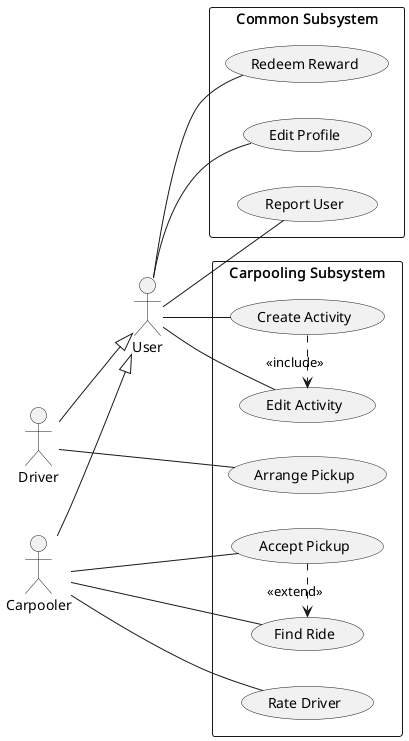
\includegraphics[width=0.8\textwidth]{use-cases-carpooling}
    \caption{Use Case Diagram 1}
\end{figure}

\begin{figure}
    \centering
    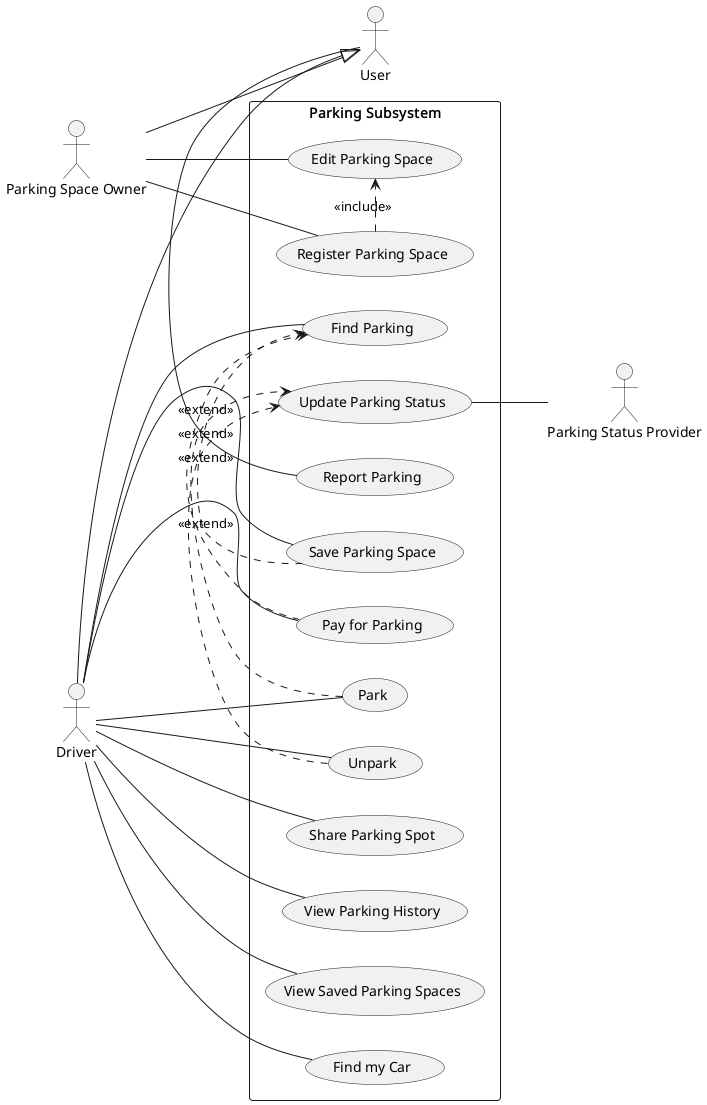
\includegraphics[width=0.8\textwidth]{use-cases-parking}
    \caption{Use Case Diagram 2}
\end{figure}

\section{Απαιτήσεις και Προδιαγραφές}

\section{Χρήση Τεχνολογιών και Εργαλείων}

\end{document}
